 The method for matching the data to a theoretical orbit described in Section \ref{sec:matchorbit} finds the best fit but it is important to know how good of a fit it is. A flat fitness curve would mean a very small change in the data could lead to a very large change in our matched orbit, i.e we have very high uncertainty. To determine the goodness of fit we vary the three parameters $\epsilon, \theta$ and $i$ separately and find the best fit for the other two parameters. In Figure \ref{fig:asymVariation} we find the best matching orbits for Particle A for asymmetries ranging from 0 to 0.2. We see that there is a clear minima around $\epsilon = 0.02$ implying that it is a good fit.
 
 In Figure \ref{fig:orbitVariation} the match of stretch 1 from measurement 1 of particle A is matched. We use the best matching asymmetry, match for orbits from the center of the pointcare map to the top. For each orbit we find the best starting position (the initial $\psi$). The result is a steady slope down to the correct orbit suggesting that this variable also had a clear best value that was chosen. 
 
 The best In Figure \ref{fig:initVariation} we use the best matching 		asymmetry and orbit for stretch 1 from measurement 1 of particle A, and the starting position (initial $\psi$) is varied over 1 full period. The relatively flat slope suggests that this parameter while certainly improving the fit slightly is not as important as the other two parameters. 
 
 \begin{figure}[H]
 \begin{center}
 \includegraphics[width=0.7\textwidth]{figures/results/particleA/A_assymVariation.pdf}
 \end{center}
 \caption{We see how the difference between the theoretical $n_z$ and all the measured  $\widetilde{n_z}$ for all measurements of particle A for different asymmetries $\epsilon$. For each asymmetry we find the orbit and the initial $\psi$ with the smallest distance for each stretch. We see that there is a clear minima around $\epsilon = 0.02$}
 \label{fig:asymVariation}
 \end{figure}
 
 \begin{figure}[H]
 \begin{center}
 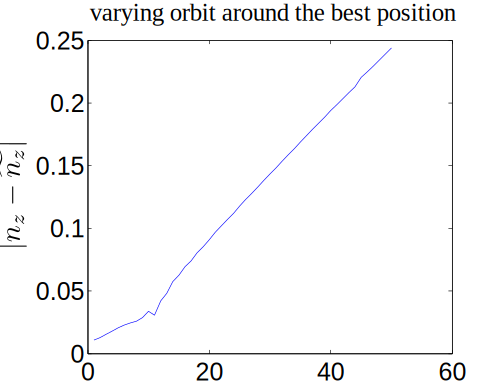
\includegraphics[width=0.7\textwidth]{figures/results/particleA/A_orbitVariation.pdf}
 \end{center}
 \caption{The difference between the theoretical $n_z$ and the measured $\widetilde{n_z}$ for the first stretch of the measurement 1 for particle A (seen in Figure \ref{fig:particleA1})with the best asymmetry for different orbits. .}
 \label{fig:orbitVariation}
 \end{figure}
 
 
 \begin{figure}[H]
 \begin{center}
 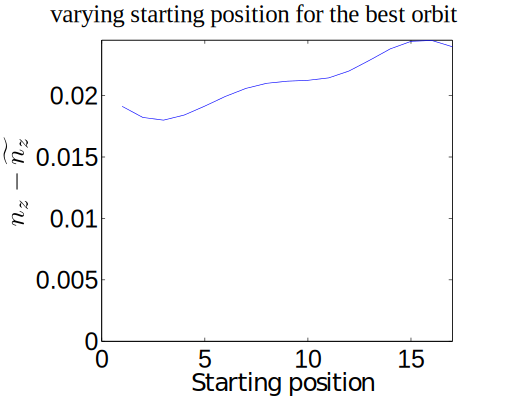
\includegraphics[width=0.7\textwidth]{figures/results/particleA/A_posVariation.pdf}
 \end{center}
 \caption{The difference between the theoretical $n_z$ and the measured $\widetilde{n_z}$ for the first stretch of the first measurement for particle A. The best orbit and best asymmetry are chosen, but different initial conditions are tested. }
 \label{fig:initVariation}
 \end{figure}
 
